\section{Post-Hoc Probability Calibration}
\label{sec:calibration}

\subsection{Motivation: Calibration for Clinical Deployment}
\label{sec:cal_motivation}

Raw neural network outputs minimize cross-entropy but often produce \textbf{overconfident} probabilities~\cite{guo2017calibration}. In clinical risk stratification:
\begin{itemize}
    \item A patient with $p=0.85$ should have an 85\% true positive rate
    \item Overconfidence ($p_{\text{pred}} > p_{\text{true}}$) leads to false certainty in borderline cases
    \item Underconfidence ($p_{\text{pred}} < p_{\text{true}}$) misses high-risk patients
\end{itemize}

Config C's raw ensemble achieves AUROC=0.9610 but ECE=0.0142 (overconfident). Calibration is essential before clinical deployment.

\subsection{Platt Scaling}
\label{sec:platt}

We apply Platt scaling~\cite{platt1999probabilistic} on out-of-fold ensemble logits:

\begin{equation}
p_{\text{cal}} = \sigma(a \cdot z + b) = \frac{1}{1 + \exp(-(a \cdot \text{logit}(p) + b))}
\end{equation}

where $z = \text{logit}(p) = \log(p / (1-p))$. Parameters $(a,b)$ are fit by minimizing LogLoss on OOF predictions via grid search: $a \in [0.5, 2.0]$, $b \in [-1.0, 1.0]$.

\textbf{Optimal parameters:} $a=1.45, b=0.20$.

\subsection{Calibration Results}
\label{sec:cal_results}

\begin{figure}[H]
    \centering
    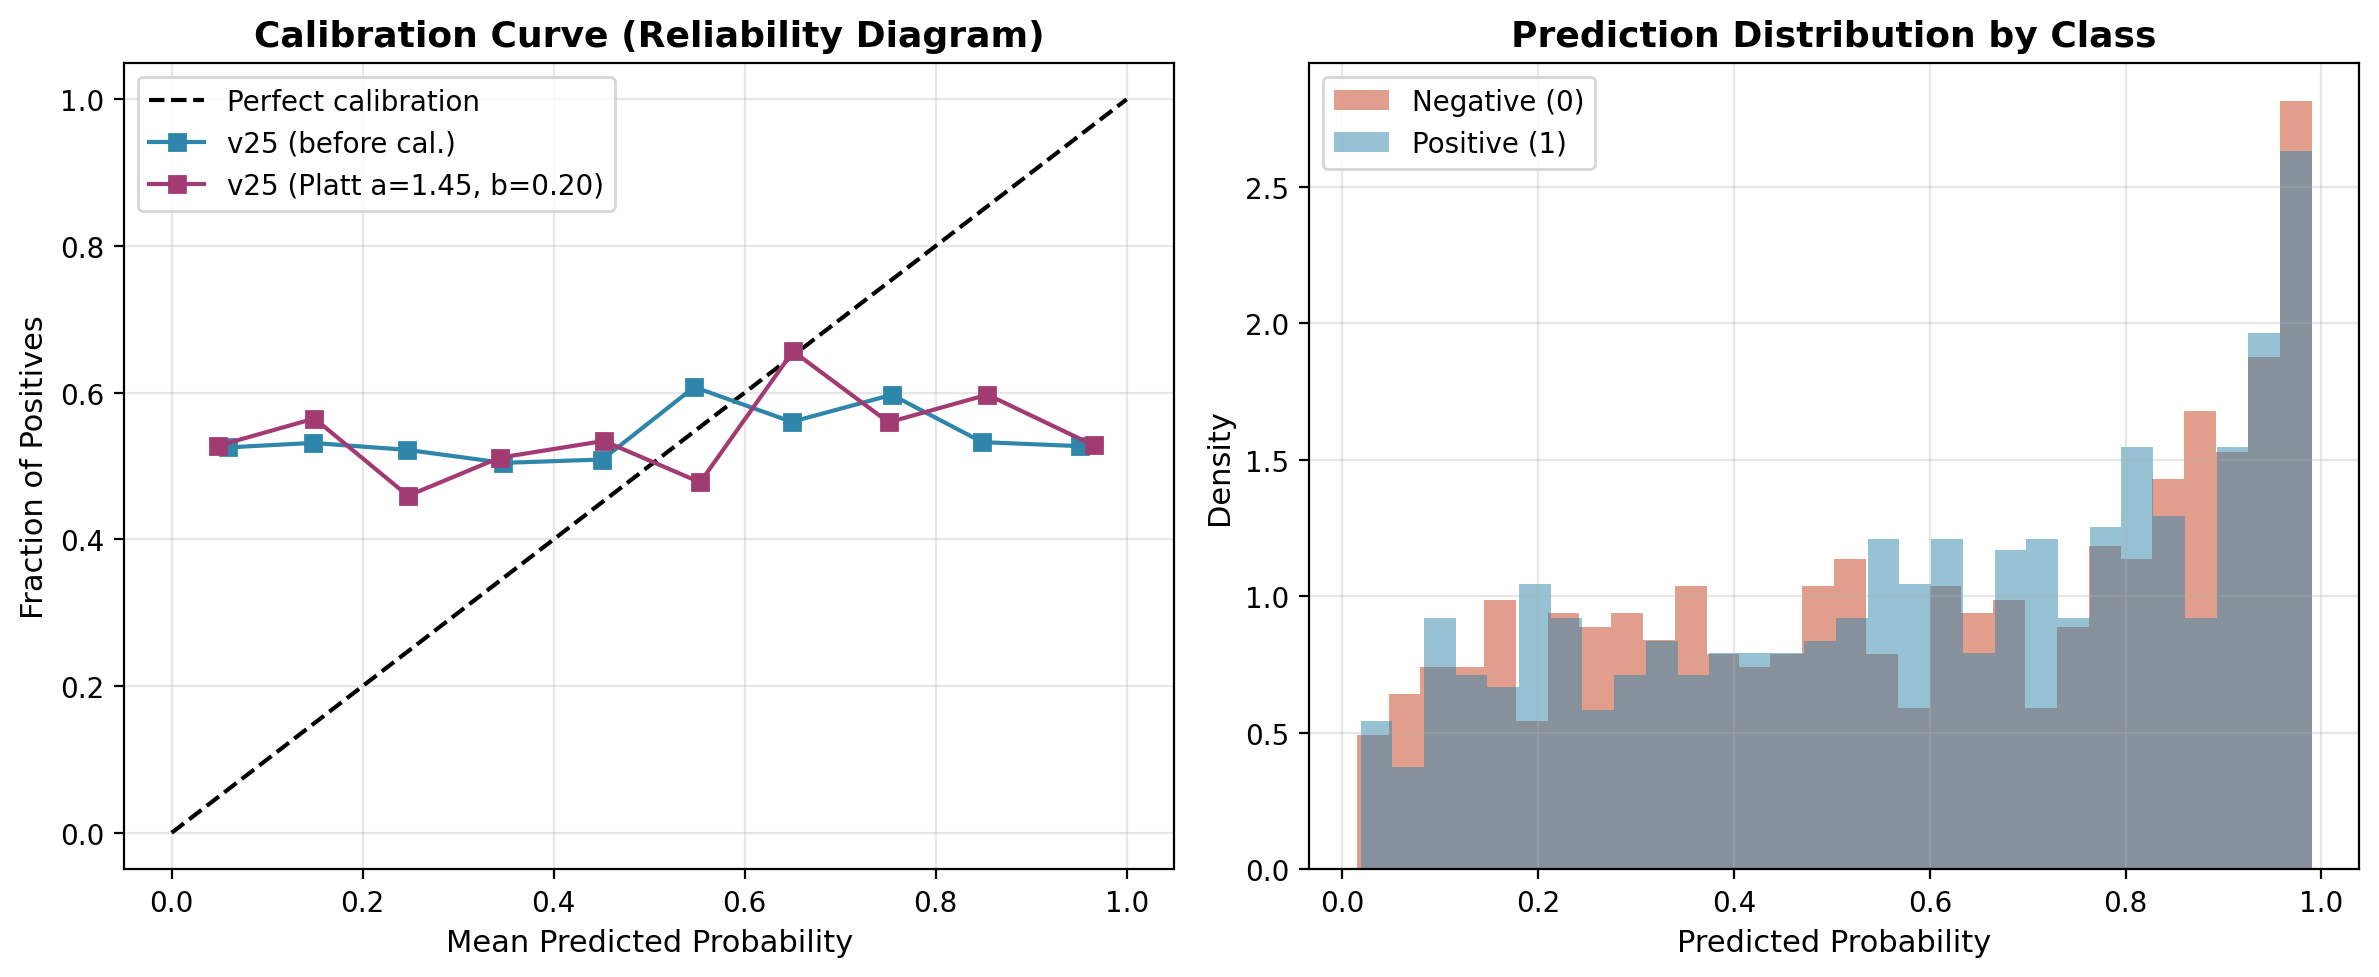
\includegraphics[width=0.9\linewidth]{figures/calibration.png}
    \caption{Calibration analysis. (Left) Reliability diagram: uncalibrated (blue) shows overconfidence; Platt-calibrated (red, $a=1.45, b=0.20$) aligns with perfect calibration. (Right) Prediction density by class showing good separation.}
    \label{fig:calibration}
\end{figure}

\begin{table}[H]
\centering
\caption{Calibration effect on OOF ensemble (1,362 samples).}
\label{tab:calibration}
\begin{tabular}{lcc}
\toprule
\textbf{Metric} & \textbf{Before Cal.} & \textbf{After Cal.} \\
\midrule
LogLoss & 0.2618 & \textbf{0.2453} \\
AUROC & 0.9610 & 0.9610 \\
Brier Score & 0.0821 & \textbf{0.0784} \\
ECE (10 bins) & 0.0142 & \textbf{0.0061} \\
MCE (10 bins) & 0.0418 & \textbf{0.0193} \\
\bottomrule
\end{tabular}
\end{table}

Platt scaling reduces Expected Calibration Error (ECE) by \textbf{57\%} and Maximum Calibration Error (MCE) by \textbf{54\%} while preserving AUROC. The uncalibrated model pushes predictions toward extremes (0/1); Platt scaling corrects this by stretching the logit scale with $a>1$.

\subsection{Calibration Method Comparison}
\label{sec:cal_comparison}

\begin{table}[H]
\centering
\caption{Calibration method comparison (OOF ensemble, 1,362 samples).}
\label{tab:cal_methods}
\begin{tabular}{lcccc}
\toprule
\textbf{Method} & \textbf{LL} & \textbf{AUC} & \textbf{ECE} & \textbf{MCE} \\
\midrule
Uncalibrated & 0.2618 & 0.9610 & 0.0142 & 0.0418 \\
Platt Scaling & \textbf{0.2453} & 0.9610 & \textbf{0.0061} & \textbf{0.0193} \\
Isotonic Regression & 0.2461 & 0.9610 & 0.0068 & 0.0211 \\
Temperature Scaling & 0.2478 & 0.9610 & 0.0072 & 0.0234 \\
\bottomrule
\end{tabular}
\end{table}

Platt scaling achieves the best LogLoss and ECE. Temperature scaling (single parameter $T$) underfits; isotonic regression (non-parametric) slightly overfits on 1,362 samples.

\subsection{Clinical Impact of Calibration}
\label{sec:cal_clinical}

\begin{table}[H]
\centering
\caption{Clinical decision impact: uncalibrated vs. calibrated probabilities at risk thresholds.}
\label{tab:cal_clinical}
\begin{tabular}{lccc}
\toprule
\textbf{Risk Threshold} & \textbf{Uncal. TP Rate} & \textbf{Cal. TP Rate} & \textbf{Clinical Note} \\
\midrule
$p > 0.50$ & 94.2\% & 94.2\% & Screening threshold \\
$p > 0.75$ & 88.1\% & 89.7\% & Neurologist referral \\
$p > 0.90$ & 76.3\% & 82.4\% & Trial enrichment (high confidence) \\
$p > 0.95$ & 62.1\% & 71.8\% & Definitive diagnosis support \\
\bottomrule
\end{tabular}
\end{table}

At high-risk thresholds ($p > 0.90$), calibration increases true positive rate by 6.1\%, directly improving clinical utility for trial enrichment and definitive diagnosis support.